% Please do not change the document class
\documentclass{scrartcl}

% Please do not change these packages
\usepackage[hidelinks]{hyperref}
\usepackage[none]{hyphenat}
\usepackage{setspace}
\doublespace




% You may add additional packages here
\usepackage{amsmath}
\usepackage{cite}
\setlength{\parindent}{4em}
\usepackage{graphicx}

% Please include a clear, concise, and descriptive title
\title{Do the benefits from early and frequent user research outweigh the potential cost on the return on investment for games?
}

% Please do not change the subtitle
\subtitle{COMP150 - Agile Development Practice}

% Please put your student number in the author field
\author{1703170}

\begin{document}

\maketitle

\abstract{One of the major factors that contribute to a games success at launch is the ability to recognise and fix problems with the game before release. But does too much user research and playtesting negatively impact development?  This paper outlines how user research is implemented using Agile development methods and how these methods affect development time and costs compared with other less rigorous methods in the games industry.  }

\section{Introduction}

User research is an incredibly important part of a games development and allows a developer to gather important data about the game [see fig.1]. But how much user research is appropriate for your game? Production teams that take an Agile approach \cite{fowler2001agile:1} to game development often implement user research early on in the process and yield positive result when implemented well [LearningGameDes], while others that prefer plan-based approaches to game development do the majority of their playtesting and user research towards the end of the development process. Often these can lead to issues at launch. The purpose of this paper is to discuss the positives and negatives of an Agile and iterative approach to game design with reference specifically to that topic of user research. The paper will compare and contrast these findings to the methodology they used in development \cite{politowski2016old,}.

\begin{center}
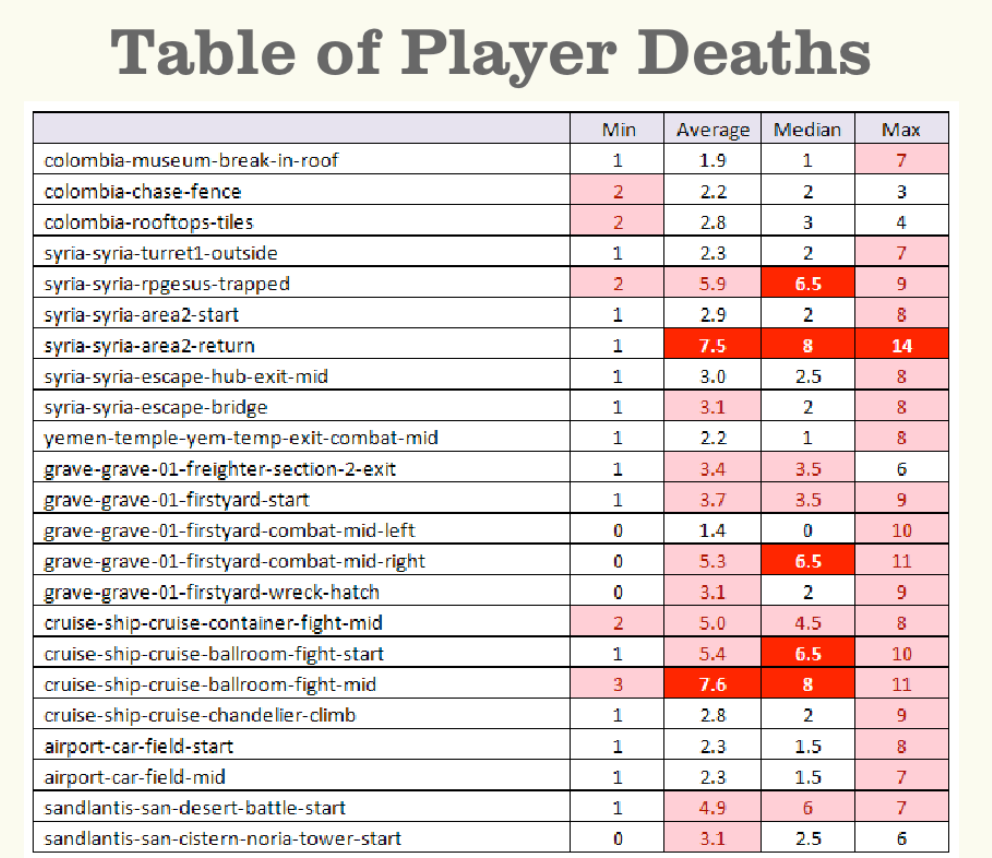
\includegraphics[scale=0.4]{PlayerDeathTable.png}
\end{center}

\begin{center}
Figure 1 [GDCAttention]
\end{center}

\section{Postmortem Comparisons}

Because in Agile, user research is done early in the development process, the data gathered from early playtesting can be used in sprint reviews and can mitigate the need for a large crunch at the end of development as bugs and design flaws can be spotted and fixed much sooner\cite{PMKOA,}. More traditional methods may not catch these in this early stage. The longer that problems go unnoticed, the more work is put into that problematic code, the more difficult and time consuming it becomes to fix later on \cite{GDCOTC,}. This clearly advocates the idea that early and often playtesting is actually beneficial with regards the development time and thus development costs. \par
In more traditional methods like waterfall, testing is usually planned to be done at the end of a project \cite{ji2011comparing,}. A lack of earlier playtesting can easily overwhelm a studio if playtesting is only used at the end of development for Quality Assurance \cite{PMTrine,}. Playtest is more about improving quality whereas QA is about getting the game to work. Only allowing for a couple of months to playtest a game before the final development stage is a risk to developers and investors. If the scope of the project has been underestimated (as can often happen in software development) then when it comes to the testing stage, a possible lack of funds or time to adequately playtest and do user research can easily become a reality\cite{PMZZ,}. As noted previously, this can mean a lot more issues at launch particularly for large AAA games [brokengamesatlaunch] or the game not being released at all. With an Agile approach, the continous iteration can ensure that a shippable build is always available and with continuous testing and feedback, each iteration is more likely to be the best the game can be at that time. This significantly lowers the risk for investors, always knowing that launch is viable \cite{ghane2017quantitative,}. This suggests that test-driven development in particular seems especially useful \cite{cunningham2005costs,}.
Day one playtesting of a game by the developers through an early prototype can also be a good way to focus the team \cite{Yampolsky:2016:LGD:2896958.2896965,}. It makes it difficult to ignore problems with the gameplay if you or other team members as developers are experiencing the issues firsthand. This works particularly well for small indie studio's who are making games with a smaller scope and constanly iterating over a basic build \cite{PMNS2,}.


\section{How early and how often?}

The question this paper asks can be seen to largely depend on how early and how often user reasearch should start. With regard to the former, it may be considered that the most appropriate time to start playtesting is as soon as the developer has a question about the game \cite{GDCSharks,}. This is likely to be very early on in the project and with Agile, and a flexible design document, user research about the game can be gathered in early iterations,. Comparatively, with plan-driven development, this is a problem because the team has a large or rigid design document, teams are less likely to want to change things before the end of development. How often a games gets playtested depends on how often content or features are integrated as well as when special events are held. Playtesting throughout gives the developer a much better grip on the players experience, saves time because developers wont be wasting time on the wrong things and gets the developer to focus on the nuances of a game. It takes time to find out what parts of a game make it the most fun \cite{GDCAED,}.


\section{The Community}

Early access on Steam is also a good way of gaining user research data\cite{GamesEA,}. 
Games that don't use Agile in some way won't be able to go Early Access, as ideally this will happen well before the game is complete. This adds another way of funding the game whilst simultaneously adding an early player base of testers who can give the developer feedback about the game while its being developed \cite{GDCOTC,}. This obviously does not suit other methods such as waterfall, which would be unable to benefit from Early Access. 
There are risks however. Let's propose for example that the initial release on Early Access isn't very appealing, with perhaps the gameplay mechanics leaving something to be desired. Normally this wouldn't be a huge problem, developers would be able to fix this in later iterations if playtesting was conducted within production. When the game has been released to the public in Early Access however, this can be an issue. The game will be judged by both players and press. People may forget about the game a few months down the line when production is finished and may not go back to see the improvements.

\section{Testing and Team Communication}

Testing early on in the development process can also be a boon to team communication as test-driven development promotes early communication between the different teams in a studio or company \cite{gallardo2009continuous,}. Communication between the Product Owner, Testers, Designers and Programmers is paramount to ensuring a successful game is made \cite{mcdaniel2015communication,}. 
Whereas if a studio elects to take a more plan-based approach or even an Agile approach with strict and inelastic procedures they may suffer \cite{cooke2012everything,} \cite{davis2012agile,}, communications may break down and team morale can be adversely affected \cite{cunningham2005costs,}. This would clearly hinder the development process as a whole and thus increase development times and costs.


\section{Conclusion}

Game development done well is inherently an iterative process and it's clear that even studios using the waterfall methodology should use iteration \cite{al2014towards,} \cite{o2015towards,}. This begs the question of whether or not user research and playtesting should be a part of that iterative process. This paper would argue that it should be. Although much of the evidence presented in this paper is anecdotal and comes out of research of various developers postmortems of their games, it is nonetheless a valuable insight into how user research is used in the development process of games today. Although using Agile doesn't mean problems can't occur in larger companies, it does appear to limit them \cite{rico2009business,} \cite{batra2010balancing,}. In the end, the findings of this paper clearly suggest that continuous playtesting and user research throughout the development process is preferable to the problems that can occur without it, especially in smaller teams and an argument can be made that larger AAA companies should also be playtesting more often, even if they opt for a more waterfall approach to production.

\bibliographystyle{ieeetran}
\bibliography{references}

\end{document}




